% Options for packages loaded elsewhere
\PassOptionsToPackage{unicode}{hyperref}
\PassOptionsToPackage{hyphens}{url}
\PassOptionsToPackage{dvipsnames,svgnames,x11names}{xcolor}
%
\documentclass[
  letterpaper,
  DIV=11,
  numbers=noendperiod]{scrartcl}

\usepackage{amsmath,amssymb}
\usepackage{iftex}
\ifPDFTeX
  \usepackage[T1]{fontenc}
  \usepackage[utf8]{inputenc}
  \usepackage{textcomp} % provide euro and other symbols
\else % if luatex or xetex
  \usepackage{unicode-math}
  \defaultfontfeatures{Scale=MatchLowercase}
  \defaultfontfeatures[\rmfamily]{Ligatures=TeX,Scale=1}
\fi
\usepackage{lmodern}
\ifPDFTeX\else  
    % xetex/luatex font selection
    \setmainfont[]{Times New Roman}
    \setsansfont[]{Times New Roman}
\fi
% Use upquote if available, for straight quotes in verbatim environments
\IfFileExists{upquote.sty}{\usepackage{upquote}}{}
\IfFileExists{microtype.sty}{% use microtype if available
  \usepackage[]{microtype}
  \UseMicrotypeSet[protrusion]{basicmath} % disable protrusion for tt fonts
}{}
\makeatletter
\@ifundefined{KOMAClassName}{% if non-KOMA class
  \IfFileExists{parskip.sty}{%
    \usepackage{parskip}
  }{% else
    \setlength{\parindent}{0pt}
    \setlength{\parskip}{6pt plus 2pt minus 1pt}}
}{% if KOMA class
  \KOMAoptions{parskip=half}}
\makeatother
\usepackage{xcolor}
\setlength{\emergencystretch}{3em} % prevent overfull lines
\setcounter{secnumdepth}{-\maxdimen} % remove section numbering
% Make \paragraph and \subparagraph free-standing
\makeatletter
\ifx\paragraph\undefined\else
  \let\oldparagraph\paragraph
  \renewcommand{\paragraph}{
    \@ifstar
      \xxxParagraphStar
      \xxxParagraphNoStar
  }
  \newcommand{\xxxParagraphStar}[1]{\oldparagraph*{#1}\mbox{}}
  \newcommand{\xxxParagraphNoStar}[1]{\oldparagraph{#1}\mbox{}}
\fi
\ifx\subparagraph\undefined\else
  \let\oldsubparagraph\subparagraph
  \renewcommand{\subparagraph}{
    \@ifstar
      \xxxSubParagraphStar
      \xxxSubParagraphNoStar
  }
  \newcommand{\xxxSubParagraphStar}[1]{\oldsubparagraph*{#1}\mbox{}}
  \newcommand{\xxxSubParagraphNoStar}[1]{\oldsubparagraph{#1}\mbox{}}
\fi
\makeatother


\providecommand{\tightlist}{%
  \setlength{\itemsep}{0pt}\setlength{\parskip}{0pt}}\usepackage{longtable,booktabs,array}
\usepackage{calc} % for calculating minipage widths
% Correct order of tables after \paragraph or \subparagraph
\usepackage{etoolbox}
\makeatletter
\patchcmd\longtable{\par}{\if@noskipsec\mbox{}\fi\par}{}{}
\makeatother
% Allow footnotes in longtable head/foot
\IfFileExists{footnotehyper.sty}{\usepackage{footnotehyper}}{\usepackage{footnote}}
\makesavenoteenv{longtable}
\usepackage{graphicx}
\makeatletter
\newsavebox\pandoc@box
\newcommand*\pandocbounded[1]{% scales image to fit in text height/width
  \sbox\pandoc@box{#1}%
  \Gscale@div\@tempa{\textheight}{\dimexpr\ht\pandoc@box+\dp\pandoc@box\relax}%
  \Gscale@div\@tempb{\linewidth}{\wd\pandoc@box}%
  \ifdim\@tempb\p@<\@tempa\p@\let\@tempa\@tempb\fi% select the smaller of both
  \ifdim\@tempa\p@<\p@\scalebox{\@tempa}{\usebox\pandoc@box}%
  \else\usebox{\pandoc@box}%
  \fi%
}
% Set default figure placement to htbp
\def\fps@figure{htbp}
\makeatother

\usepackage{booktabs}
\usepackage{longtable}
\usepackage{array}
\usepackage{multirow}
\usepackage{wrapfig}
\usepackage{float}
\usepackage{colortbl}
\usepackage{pdflscape}
\usepackage{tabu}
\usepackage{threeparttable}
\usepackage{threeparttablex}
\usepackage[normalem]{ulem}
\usepackage{makecell}
\usepackage{xcolor}
\KOMAoption{captions}{tableheading}
\makeatletter
\@ifpackageloaded{caption}{}{\usepackage{caption}}
\AtBeginDocument{%
\ifdefined\contentsname
  \renewcommand*\contentsname{Table of contents}
\else
  \newcommand\contentsname{Table of contents}
\fi
\ifdefined\listfigurename
  \renewcommand*\listfigurename{List of Figures}
\else
  \newcommand\listfigurename{List of Figures}
\fi
\ifdefined\listtablename
  \renewcommand*\listtablename{List of Tables}
\else
  \newcommand\listtablename{List of Tables}
\fi
\ifdefined\figurename
  \renewcommand*\figurename{Figure}
\else
  \newcommand\figurename{Figure}
\fi
\ifdefined\tablename
  \renewcommand*\tablename{Table}
\else
  \newcommand\tablename{Table}
\fi
}
\@ifpackageloaded{float}{}{\usepackage{float}}
\floatstyle{ruled}
\@ifundefined{c@chapter}{\newfloat{codelisting}{h}{lop}}{\newfloat{codelisting}{h}{lop}[chapter]}
\floatname{codelisting}{Listing}
\newcommand*\listoflistings{\listof{codelisting}{List of Listings}}
\makeatother
\makeatletter
\makeatother
\makeatletter
\@ifpackageloaded{caption}{}{\usepackage{caption}}
\@ifpackageloaded{subcaption}{}{\usepackage{subcaption}}
\makeatother

\usepackage{bookmark}

\IfFileExists{xurl.sty}{\usepackage{xurl}}{} % add URL line breaks if available
\urlstyle{same} % disable monospaced font for URLs
\hypersetup{
  pdftitle={v2},
  pdfauthor={Maiko Hata},
  colorlinks=true,
  linkcolor={blue},
  filecolor={Maroon},
  citecolor={Blue},
  urlcolor={Blue},
  pdfcreator={LaTeX via pandoc}}


\title{v2}
\author{Maiko Hata}
\date{}

\begin{document}
\maketitle


A. Table of 10 exit reasons

\begin{longtable}[l]{ll}
\caption{Table of Exit Reasons}\\
\toprule
Exit Reasons & Exit Category Codes\\
\midrule
Program completion & Category (C) 1: A child is no longer eligible for Part C prior to reaching age three \\
Exit at age three & C2: A child is exiting Part C and has been determined to be eligible for Part B \\
Exit at age three & C3: Part B eligible, continuing in Part C  \\
Exit at age three & C4: Not eligible for Part B, exit with referrals to other programs \\
Exit at age three & C5: Not eligible for Part B, exit with no referrals \\
\addlinespace
Exit at age three & C6: Part B eligibility not determined \\
Not receiving services  & C7: Deceased\\
Not receiving services  & C8: Moved out of state \\
Not receiving services  & C9: Withdrawal by parent (or guardian) \\
Not receiving services  & C10: Attempts to contact the parents and/or child were unsuccessful \\
\bottomrule
\end{longtable}

B. National and Oregon CHILD COUNTS

NOTE TO SELF: ADD THE CENSUS NUMBER FOR FINAL PROJECT! BIND\_ROWS!! WEEK
2? 3? Labs.

B-1. Load data

B-2: chart 1

\begin{longtable}[l]{llllllll}
\caption{Child Count (US & Oregon)}\\
\toprule
State & American Indian or Alaska Native (\%) & Asian (\%) & Black or African American (\%) & Hispanic/Latino (\%) & Native Hawaiian or Pacific Islander (\%) & Two or More Races (\%) & White (\%)\\
\midrule
Oregon & 0.87 & 3.27 & 2.69 & 22.77 & 0.3 & 5.41 & 64.69\\
US and Outlying Areas & 0.69 & 4.3899999999999997 & 12.35 & 27.65 & 0.3 & 4.2300000000000004 & 50.38\\
\bottomrule
\end{longtable}

B-2: visualization 1

\begin{verbatim}
 chr [1:14] "0.87" "0.69" "3.27" "4.3899999999999997" "2.69" "12.35" ...
\end{verbatim}

\pandocbounded{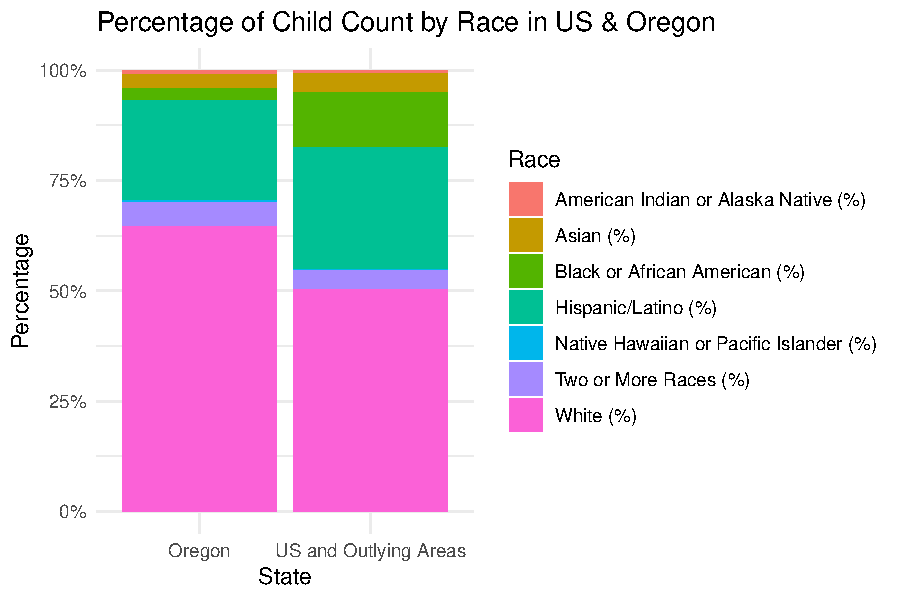
\includegraphics[keepaspectratio]{v2_files/figure-pdf/unnamed-chunk-14-1.pdf}}

\pandocbounded{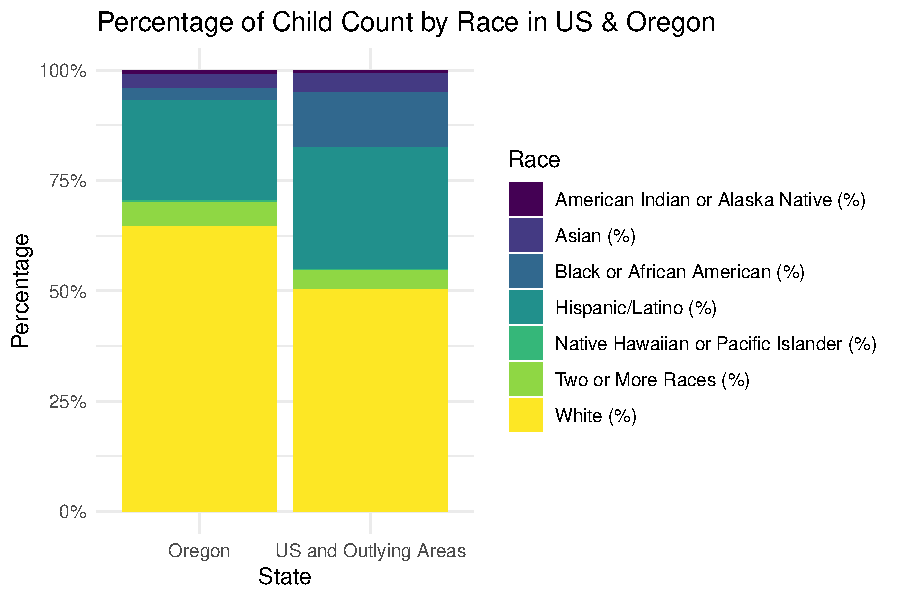
\includegraphics[keepaspectratio]{v2_files/figure-pdf/unnamed-chunk-15-1.pdf}}

\pandocbounded{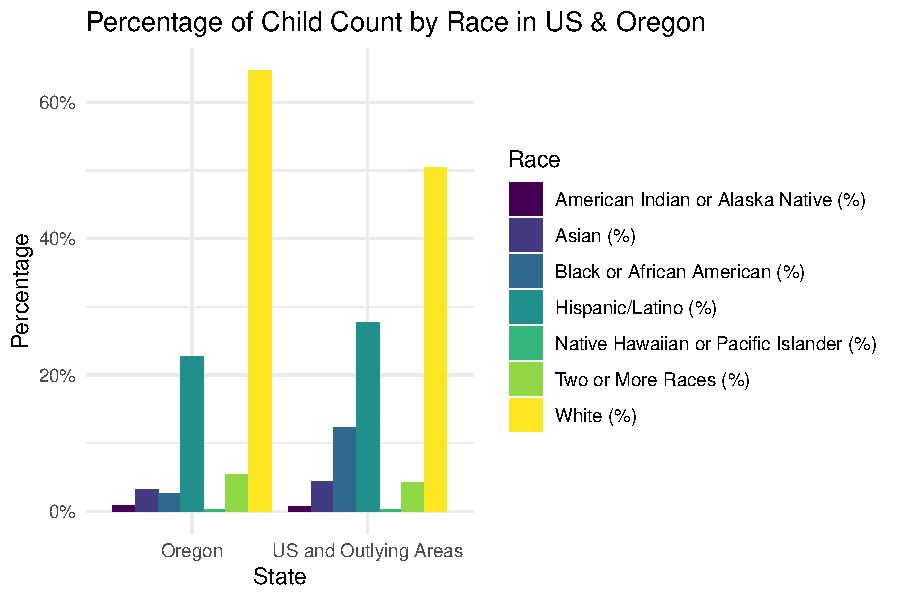
\includegraphics[keepaspectratio]{v2_files/figure-pdf/unnamed-chunk-16-1.pdf}}

C. National and Oregon EXIT data by RACE

C. Oregon data by LANGUAGES

\begin{longtable}[l]{lrrrrrr}
\caption{Initial Oregon Data by Home Languages}\\
\toprule
primary\_language & exit\_total & withdrawal\_by\_parent & attempts\_to\_contact\_unsuccessful & moved\_out\_of\_state & part\_b\_eligible\_exiting\_part\_c & complete\_or\_not\_eligible\\
\midrule
Chinese & 19 & 2 & 1 & 2 & 12 & 2\\
English & 16528 & 3088 & 1318 & 862 & 9326 & 1701\\
Other languages & 2725 & 501 & 183 & 209 & 1565 & 227\\
Russian & 35 & 10 & 2 & 5 & 16 & 1\\
Sign languages & 7 & 0 & 0 & 3 & 4 & 0\\
\addlinespace
Spanish & 2068 & 266 & 184 & 53 & 1388 & 150\\
Vietnamese & 67 & 15 & 4 & 6 & 41 & 1\\
NA & NA & NA & NA & NA & NA & NA\\
\bottomrule
\end{longtable}




\end{document}
